\chapter{Introduction}\label{chap:intro} 
    A sudoku puzzle is a popular logic-based game where any player should fill an $n \times n$ grid while following the rules. The rule includes putting all numbers from 1 to n without repetition to row, column, and subgrid. The size of the common puzzle used by anyone today is $9 \times 9$ which consists of a subgrid of a size $3 \times 3$. However, there are also existing puzzles with different sizes such as $6 \times 6$, $12 \times 12$, $16 \times 16$, and $25 \times 25$. Increasing the puzzle size also increases the complexity and the computational load. The valid Sudoku solution must simultaneously satisfy multiple interdependent constraints and that is the reason why it belongs to the constraint satisfaction problem~\cite{lloyd2020, simonis2005sudoku,eppstein2006computational,yato2003complexity}. 


    There are already existing algorithms which efficiently solve small instances like the traditional rule-based algorithm and the backtracking algorithm. However, these algorithms tend to struggle and often give invalid solutions for larger puzzle sizes~\cite{is2012techniques}. Because of these challenges, a lot of heuristic methods were introduced and developed. These new methods propose a new approach and that is guiding the process of searching for a valid solution to promising regions of the solution space instead of trying to explore all possibilities and doing an exhaustive search. The constraint propagation is one of those methods which gained attention from researchers because of its effectiveness. It eliminates any infeasible candidate leading to a more promising search space.~\cite{lloyd2020}.

    As the algorithms found its way to improve in response to more complex sudoku puzzles, metaheuristic algorithms were developed. These algorithms were designed to achieve optimal solutions through repetitive refinement. Because of this, it became powerful alternatives to existing algorithms and some researchers even combined this to existing algorithms to build a better sudoku solver. Some examples of these algorithms are Artificial Bee Colony, Particle Swarm Optimization, Genetic Algorithm, and Ant Colony Optimization. Instead of deterministic search, their way of finding an optimal solution is through collective intelligence and feedback. The ant colony optimization algorithm is inspired from the foraging behavior of ants in the real world. It was also one of the most well-known swarm-based algorithms when it comes to solving combinatorial problems. The main feature of ACO is its pheromone-based feedback and its probabilistic exploration which makes it suitable for solving constraints-based problems like Sudoku.~\cite{dorigo1992}.

    However, the implementation of the traditional ACO is sequential. This often raises an issue when it comes to increasing the complexity of the problem. As the complexity of the problem increases, ants are likely to have difficulty in converging to a complete solution thus leading to invalid solutions. In the context of Sudoku, increased execution time and invalid Sudoku solutions are the common performance of the ACO because of its limited exploration in the solution space. To overcome this challenges, this research proposes a Multithreaded Multi-Colony Ant Optimization with Ring and Random Communication Topologies that adapts the constraint propagation for early removable of infeasible solutions, dynamic collaborative multi-colony and thread communication mechanism for a wider exploration in the solution space and adaptive cooperation for faster realization of a valid Sudoku solution. This proposed model is designed to be more efficient in solving large and complex sudoku puzzles where existing sudoku solvers often fail. This research ensures that there is balance between the exploration and exploitation mechanism. 

\section{Background of the Study}\label{sec:Background}

\subsubsection{Deterministic Approach}
    Historically, deterministic approach was the first option to solve sudoku puzzles. It mainly uses the backtracking algorithms as shown in Figure~\ref{backtrack}. It goes by filling cells with valid values then backtrack if it leads to invalid puzzle~\cite{norvig2006solving}~\cite{Schott}~\cite{bhattarai2025study}. Since the search space is very large, this approach suffers from poor performance especially when it comes to hard puzzles. Since it does not know whether a certain assignments leads to invalid solution, this algorithm tends to face thousands of dead-ends~\cite{eppstein2006computational}. 

    \begin{figure}[H]
        
\includegraphics[width=\textwidth]{../figures/Backtrack_Back.png}
        \centering
        \caption{Backtracking Algorithm}\label{backtrack}
    \end{figure}

\subsubsection{Heuristic Approaches}
    To address the brute-force characteristics of the backtracking algorithm, heuristic approaches were introduced as shown in Figure~\ref{heuristic}. These approaches eliminate invalid values before the guessing starts such as naked and hidden singles~\cite{crook2009pencil}~\cite{bhattarai2025study}. Because of this, the search space was reduced and the guessing is within the valid assignments. However when it comes to complex sudoku, it often goes back to brute-force if there are no naked or hidden singles anymore. 

    \begin{figure}[H]
        
\includegraphics[width=\textwidth]{../figures/Hueristic_Back.png}
        \centering
        \caption{Hueristic Approach}
        \label{heuristic}
    \end{figure}

\subsubsection{Metaheuristic Approaches}
    As researchers continue to address the limits of the previous algorithms, metaheuristics approaches were introduced specifically swarm-based algorithm as shown in Figure~\ref{swarm}. As these approaches are designed to find a solution stochastically, they can avoid getting trapped in local optima~\cite{mantere2007solving}. Genetic Algorithms (GA), Simulated Annealing (SA), and Particle Swarm Optimization (PSO) are examples of these metaheuristic approaches. However, Ant Colony Optimization (ACO) gains popularity in solving constraint satisfaction problems. Dorigo~\cite{dorigo1992} proposed this ACO which is inspired by foraging behaviour of real ants. The ants leave pheromone trails to paths they took. Instead of brute-force, ants, eventually, converge on a solution based on feedback~\cite{dorigo2004ant}

    \begin{figure}[H]
        
\includegraphics[width=\textwidth]{../figures/Swarm_Back.png}
        \centering
        \caption{Swarm-Based Algorithm}\label{swarm}
    \end{figure}

\subsubsection{Parallel ACO}
    As the ACO gained popularity due to its performance, performance was being questioned because of its sequential implementation. This leads to the interest of many to explore parallelism of ACO. Pedemontal et al.~\cite{pedemonte2011bit}~\cite{randall2002} demonstrated parallel ants where ants can construct their solution independently. In the work of Yang and Fang~\cite{yang2015}, they introduced a framework where parallel colonies of ants communicate promoting a global convergence as shown in Figure~\ref{parallel}. This approach ensures that every corner of the solution space is explored. 

    \begin{figure}[H]
        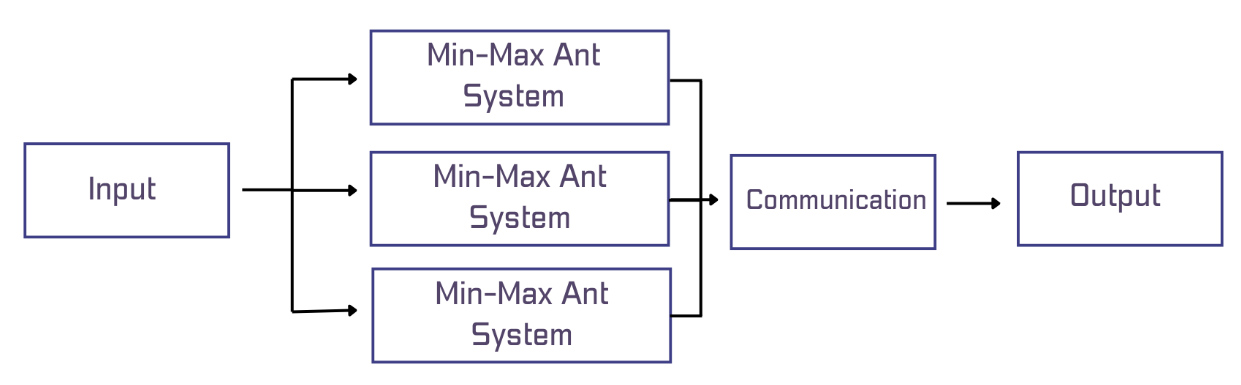
\includegraphics[width=\textwidth]{../figures/ParallelACO_Back.png}
        \centering
        \caption{Randomly Matched Parallel Ant Colony Optimization}\label{parallel}
    \end{figure}


\section{Problem Statement}\label{sec:Problem}

Solving sudoku puzzles, especially larger puzzle sizes, is very expensive when it comes to computational cost. It is because each cell must satisfy interdependent constraints. Existing implementation of heuristic and metaheuristics algorithms faces challenges when they are introduced to large and complex sudoku puzzles. Figure~\ref{base_solver} shows integration of CP and ACS as sudoku solver. However, single-colony ACS implementations are efficient for smaller sizes of sudoku but still having difficulties in solving larger puzzle sizes. It is because the pheromone intensifies often only on the selected paths leading to stagnation and making the search process stuck on a certain region of the search space~\cite{dorigo1992, lloyd2020}. 
    
\begin{figure}[H]
        
\includegraphics[width=\textwidth]{../figures/CP-ACS.png}
        \centering
        \caption{CP-ACS of Lloyd and Amos~\cite{lloyd2020}}\label{base_solver}
    \end{figure}

Some approach used multi-colony model instead of relying to a single-colony. The Dynamic Collaborative Multi-Colony ACO (DCM-ACO) framework where colonies exchange pheromone information based on their performance~\cite{mo2022} is applied to Travelling Salesman Problem (TSP). But the periodic communication between colonies often results in early convergence thus reducing diversity when introduced to larger and more complex sudoku puzzles.  

Similarly, to address the sequential process of the ACO, parallel implementation was developed. However, it was applied to travelling salesman problem (TSP). In the work of Randall and Lewis~\cite{randall2002}, it proposes a master-slave parallelization in which the master processor is the one responsible for collecting, sorting, and distribution of solutions from and to the slave processors. This framework gives heavy load to the master processor which in turn results in high computational time. The process of solving Sudoku puzzles is computationally expensive because each single cell in the grid has to satisfy many simultaneous constraints. Even though heuristic and metaheuristic algorithms have successfully improved solution efficiency, the current implementations still face significant challenges regarding scalability, convergence speed, and workload balance.

    \begin{figure}[H]
        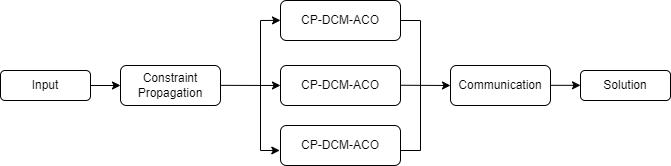
\includegraphics[width=\textwidth]{../figures/Proposed Solver SOP.png}
        \centering
        \caption{Proposed Sudoku Solver}\label{proposed solver}
    \end{figure}

This research develops  a multi-threaded multi-colony ant optimization with ring and random communication topologies to address these challenges. Furthermore, this study fills the gap of extending the RMACO, who uses a single colony per processor, into a collaborative multi-colony ant optimization for each processor. This framework, originally applied to TSP domain, is used in the domain of constraint satisfaction problem specifically Sudoku. The model combines the constraint propagation which removes infeasible solutions, the DCM-ACO for exchanging pheromone information between colonies, and communication topologies adapted from RMACO between threads to maintain diversity as shown in Figure~\ref{proposed solver}. The model is designed to handle even larger and more complex sudoku puzzles.


\section{Aim of the Work}\label{sec:Aim}
    \subsection{General Objective}
        This study aims to deploy a web-based sudoku solver that uses a multithreaded multi-colony ant optimization with ring and random communication topologies. 
    \subsection{Specific Objectives}
        \begin{enumerate}
            \item Implement multiple multi-colony ant optimization (CP-DCM-ACO) solvers running concurrently in separate threads with ring and random communication topologies.
            \item Perform an ablation study to compare different combination of parameters for the enhancement of the model's performance. 
            \item Perform state-of-the-art comparative analysis between the proposed sudoku solver and existing Sudoku-solving algorithms, including the baseline, CP-DCM-ACO, based on success rate, average completion time, and average number of iterations it takes to generate a solution.
            \item Deploy a web-based application that will enable users to generate their own Sudoku puzzles and find solutions using the proposed multithreaded sudoku solver.
        \end{enumerate}
    
        \subsection{Scope and Limitations}
            This research is focused on the design and performance of the proposed multi-threaded multi-colony ant optimization with ring and random communication topologies for solving a logic-based combinatorial problem which is the sudoku. The base solver of the proposed model is CP-DCM-ACO which is run by multiple threads concurrently. Each thread acts like an independent solver but communicates with other threads periodically. The proposed model is compared with existing sudoku solvers and its performance is evaluated based on solution success rate, average completion time, standard deviation, and the average number of iterations to generate a solution. Different sizes of sudoku are used like $6 \times 6$, $9 \times 9$, $12 \times 12$, $16 \times 16$, and $25 \times 25$ to show the robustness and the scalability of the model in increasing complexity and difficulty levels. A web-based application will be deployed allowing users to input their own sudoku puzzles which will be solved by the proposed model thus creating an interactive environment. 
    
            Although there are other combinatorial problems, this study is limited to sudoku puzzles only. However, this proposed model might be implemented to solve other combinatorial problems but such notion is beyond the scope of this research. Furthermore, the implementation of the proposed model is within the environment of multi-core CPU and does not wish to use GPU-based architectures. 


        \subsection{Significance of the Study}
            The proposed multithreaded multi-colony ant optimization with ring and random communication topologies proved contribution when it comes to the field of constraint-based optimization and enhancement of metaheuristics algorithms. Theoretically, this research improves the base model which is the CP-DCM-ACO by introducing a multithread with inter-thread collaboration framework allowing each independent instance of a solver to exchange valuable information. This helps improve the scalability of the model as it balances the exploration and exploitation mechanism without centralized control. 

            The integration of constraint propagation, dynamic collaborative multi-colony ant, and collaboration between threads contributes to a paradigm of efficient communication in shared-memory environments. This can provide deeper understanding on further optimization of swarm-based algorithms in modern multi-core processors. The current results can be a basis for future contribution to parallel metaheuristics, specifically swarm-based algorithms and also to collaborative multi-agent frameworks. In practical terms, this proposed model contributes to the need for a faster and more reliable framework for solving combinatorial problems. Sudoku, as the representative of the logic-based combinatorial problems, provides clear indication about how the proposed model handles complex and interdependent constraints.

            Overall, this study carries significance on the development of metaheuristic algorithms in terms of efficiency and adaptability. The proposed framework not only provides a clear demonstration of how the cooperation between threads in a multithreading environment can be used to solve real-world constraint-driven problems but also expands the boundaries of swarm-based optimization algorithms. 

\section{Theoretical and Conceptual Framework}\label{sec:Framework}

\begin{center}
    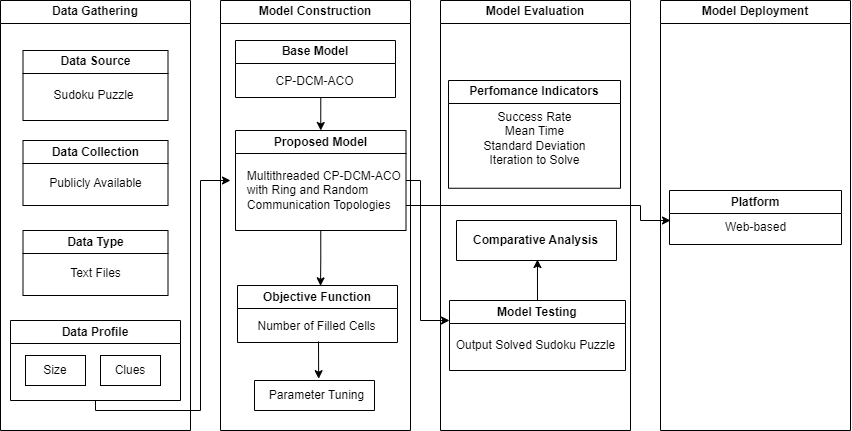
\includegraphics[width=\linewidth]{../figures/Theoretical and Conceptual Framework.png}
    \captionof{figure}{Theoretical and conceptual framework}
    \label{framework}
\end{center}
  

    Figure~\ref{framework} shows the Theoretical and Conceptual Framework which follows the general approach of the study. The theoretical foundation of this study is based on the integration of the constraint propagation, dynamic collaborative multi-colony ant optimization, and the communication designed for multi-thread environments. Sudoku puzzles used in this study are publicly available and stored in text format. The sudoku puzzles are in different sizes with different numbers of clues in it which determine its difficulty. These collected datasets will be the input for the model.

    First, the constraint propagation is the first one who receives the input. It eliminates infeasible values for cells in the sudoku puzzle in order to reduce the search space and remove invalid solutions. The base model which is the CP-DCM-ACO then receives the output from the initial pass of the constraint propagation. Different colonies here share pheromone information based on their performance. The multithreaded framework allows multiple base models, CP-DCM-ACO, to run in multiple threads separately.  The communication between threads enables sharing of valuable information between threads to prevent stagnation and increase diversity. The number of correctly filled cells is what defines the objective function in this proposed model. 

    To evaluate the performance of the proposed model, performance metrics are declared such as solution success rate, average completion time, standard deviation, and average number of iterations to generate a valid sudoku solution. These performance metrics are also applied to other sudoku solvers including the base model, CP-DCM-ACO, to have a clear comparison between the proposed model and the existing sudoku solvers. Lastly, the study deploys the proposed model as a web application allowing user interaction and showcasing the proposed model’s performance and functionality. 





